\documentclass[a4paper,12pt]{article}

\usepackage{masterArticle}


\begin{document}

\title{Создание набора инструментов для поиска электронных книг в~Интернете.\\
Серверная~часть, 
обеспечивающая хранение информации о~книгах, поиск по ней и возможность модифицировать её.}
\author{Иваницкий Андрей}
\date{\today}
\maketitle

\newpage


\begin{center}
\textbf{Реферат}
\end{center}

Мотивацией для данного проекта послужило желание облегчить работу пользователей с электронными книгами. Ресурсы, которые сейчас есть в Интернете, позволяют пользователю последовательно сначала находить нужную книгу, затем самостоятельно скачивать и искать программу, которая может работать с файлом в заданном формате.

Основная идея проекта --- избавить пользователя от лишних и трудоемких действий, оставив ему самую приятную часть --- непосредственно чтение книги. Таким образом, проект призван объединить все стадии подготовки к чтению (поиск, скачивание, открытие файла) в одну.

В этом проекте реализована внутренняя часть веб-сервера.
С помощью Sphinx реализован мощный быстрый поиск по информации, хранящейся в базе на сервере.
Удовлетворены все требования, предъявленные к поисковому механизму.
Реализован гибкий, расширяемый протокол взаимодейсвтия с анализатором.


\newpage
\tableofcontents
\newpage


\section{Введение}
В последние годы влияние Интернета на жизнь человека становится все сильнее. Это обусловлено тем, что Интернет предоставляет гораздо больше удобства и возможностей для доступа к информации. Не оказалась в стороне от Интернета и такая важная часть работы и досуга, как чтение книг.

Двадцать лет назад для того, чтобы найти книгу человек шел в библиотеку или в книжный магазин. Если он искал определённую книгу -- достаточно было назвать фамилию автора и название книги, а порой даже одного названия было достаточно. Если же выбор книги ещё не был сделан, всегда можно было получить помощь от сотрудника магазина или библиотеки. Сегодня ситуация с библиотеками и книжными магазинами изменилась несильно, но наравне с бумажными книгами появилась возможность читать книги в электронном виде. 

Большое количество книг оцифровано и хранится в сети Интернет, многие из них находятся в свободном доступе. С одной стороны, это должно упрощать процесс получения книг, \tk теперь они стали доступны из любого места, где есть возможность выхода в Интернет. С другой стороны, перед пользователем встает новые проблемы. Во-первых, теперь ему необходимо самому искать книгу в сети, где количество информации растет с каждым днем. Во-вторых, после того, как он нашел нужную книгу -- ее нужно скачать, а затем найти программу, которая позволяет читать файл в найденном формате. 

%TODO 
На настоящий момент в Интернете существует множество электронных библиотек, поиск по которым весьма затруднен из-за того, что не существует системы, которая могла бы объединить всю информацию с этих библиотек. Следовательно, пользователям приходится либо искать в каждой из электронных библиотек в отдельности, либо пользоваться существующими поисковыми системами. Есть еще одна проблема, связанная с наличием большого количества электронных библиотек. Она состоит в том, что единый формат для предоставления информации о книгах появился только недавно, поэтому каждая библиотека предоставляет свой формат.

У существующих поисковых систем, в свою очередь,  есть одна очень важная особенность -- они обладают ограниченными возможностями в проведении специализированного поиска в сети. Поэтому в результате поиска пользователь получает всю информацию, которая соответствует поисковому запросу и дальше уже начинается работа самого пользователя над тем, чтобы эту информацию профильтровать и извлечь оттуда именно то, что ему нужно. 

Таким образом, выявляются две важные проблемы, затрудняющие поиск книг. Первая проблема -- различные библиотеки имеют разные интерфейсы, вторая -- существует множество форматов, в которых может быть представлена электронная книга. 

В данной работе была разработана система, упрощающая задачу поиска, чтения и управления книгами. 


\section{Обзор существующих решений}

Все эти проблемы не новы и попытки решить эти проблемы уже предпринимались.

Например, широко известная поисковая система Google предоставляет свой сервис для поиска электронных книг -- Google books (\url{http://books.google.com}). Этот сервис выполняет полнотекстовый поиск по книгам, которые Google сканирует и сохраняет в своей базе данных. В качестве результатов поиска выдается большое количество информации о самой книге, о различных изданиях этой книги и ссылки на ресурсы, где пользователь может приобрести книгу. Благодаря полнотекстовому поиску  по содержанию, есть возможность найти книгу, имея сильно ограниченное количество информации о ней. Этот сервис не решает ни проблему унифицированного доступа к информации о книгах, ни проблему различных форматов книг.

Сайт \url{http://ebdb.ru}(electronics books data base)  -- это поисковая система, которая обходит интернет и сохраняет у себя ссылки на те страницы сторонних ресурсов, которые содержат ссылки на книги. В результате поиска выдается список ссылок на страницы, содержащие книги. Для того, чтобы получить книгу пользователь должен перейти по ссылке, и, возможно, зарегистрироваться на ресурсе. Это решает проблему поиска книг, находящихся в свободном доступе, но остаются другие задачи, которые пользователь вынужден выполнять самостоятельно (скачивание книг и поиск подходящей программы для просмотра). Эта поисковая система тоже не решает проблемы унифицированного доступа и проблему различных форматов книг.

Есть большие системы, решающие проблему унифицированного доступа и различных форматов книг, а именно, Amazon Kindle, Sony Reader и подобные. 
Это программно-аппаратные платформы для чтения электронных книг. Они предоставляют устройство, которое имеет доступ к определенному хранилищу. Пользователь может подключить свое устройство к Интернету, найти нужную книгу в этом хранилище и купить ее. Дальше устройство само скачает книгу и откроет ее.
Из минусов у таких систем то, что эти системы платные и зависимые от устройства. Количество доступных книг -- ограничено теми книгами, которые хранят/продают хранилища, к которым они подключаются. Но это не единственные минусы таких систем. Так, к примеру, у Amazon Kindle за каждый загруженный текст (вне зависимости от источника загрузки) требуется заплатить компании Amazon от 10 центов. Еще Amazon контролирует информацию, содержащуюся на устройствах, находящихся у пользователей и по своему усмотрению удаляет её (в том числе книги, приобретённые непосредственно у Amazon).

Существует открытая технология, решающая проблему унифицированного доступа  -- OPDS (Open Publication Distribution System).
OPDS -- это новый активно развивающийся стандарт, который построен на базе расширяемого языка разметки Atom. Этот стандарт был специально разработан для предоставления информации об электронных документах. В нем учтены особенности такого рода информации (наличие аннотации, автора, изображения обложки и пр.).
Основная идея существования такого стандарта в том, что если многие сайты будут распостранять свою информацию о книгах в таком формате, то клиентские программы могут работать с ними единообразно (см. \picref{fig:scheme}). Несмотря на то, что стандарт появился недавно, уже существуют сайты и клиетские программы, использующие этот протокол. 

\begin{figure}
\centering
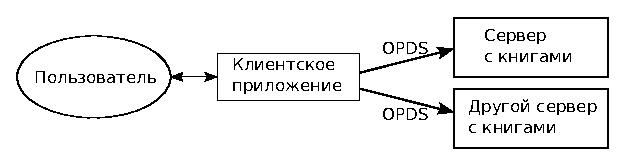
\includegraphics[width=.5\textwidth]{scheme}
\caption{Схема взаимодействия с использованием формата OPDS}\label{fig:scheme}
\end{figure}

Одим из самых крупных сайтов, предоставляющих информацию по протоколу OPDS, является BookServer (\url{http://bookserver.archive.org}).
Этот некоммерческий проект является частью проекта Internet Archive (\url{http://archive.org}) и является универсальной и открытой системой распостранения электронных книг. BookServer это архитектура, объединяющая различные форматы книг, конвертируя их, при необходимости, в нужный формат. Система обеспечивает каталогизацию книг, имеющихся в магазинах, библиотеках или в открытом доступе. Электронный текст можно прочитать на любом конечном устройстве, будь то нетбук, смартфон или специализированное устройство для чтения, наподобие Kindle. Хотя сайтом уже можно пользоваться, он еще находится на стадии разработки, с чем, вероятно, связано отсутствие расширенного поиска по книгам, фильтрации по языкам/жанрам. Так же, минусом этого проекта для русскоговорящих пользователей является невозможность поиска с использованием русских символов.

%TODO BEGIN
\section{Описание системы в целом}
Проект состоит из серверной и клиентской частей.

Серверная часть собирает в сети Интернет информацию об электронных книгах и представляет собранную информацию для обычных пользователей в виде web-интерфейса и для клиентских программ -- в формате OPDS.

Клиентская часть представляет собой программу для удобной работы с сервером, предоставляющим по запросам информацию в формате OPDS. Клиент должен работать как с "родным" сервером, так и с другими серверами, поддерживающими OPDS, например feedbooks.com.

Серверная часть проекта состоит из 3 подпроектов:
\begin{itemize}
	\item собственно web-сервер, включающий базу данных, поиск по ней, представление информации в web и opds форматах (python, django)
	\item сборщик информации в сети (crawler) (java)
	\item анализатор найденной информации, разбирающий информацию о книгах (java) 
\end{itemize}
Клиентских программ написано 2:
\begin{itemize}
	\item На С++ (с интерфейсом Qt)
	\item На Java 
\end{itemize}

Клиентская программа на Java более переносима, но для нее необходимо на девайсе иметь java-машину. В свою очердь программа на Qt не требует установки никаких дополнительных библиотек, работает быстрее, но переносимость ниже, чем у java.
		
\section{Описание компонентов системы и их взаимодействие}

% Может стоит вставить пару картинок

Пользователь устанавливает у себя на машине одну из клиентских программ. При поиске книги программа обращается к одному из серверов, поддерживающих протокол OPDS,(OpenSearch?). Сервер обрабатывает запрос, и возвращает данные в в нужном формате. 
% TODO STOP

%

\section{Постановка задачи}

\subsection{Хранение данных}

Необходимо хранить информацию о книгах

\subsection{Поиск по данным}

Если существует некоторая большая база с информацией, то очевидно, 
что для быстрой и удобной работы с ней необходим мощный, быстрый и удобный поиск.

В нашей модели для пользователя есть несколько сущностей: название книги, 
список её авторов, язык, на котором написана книга, тэги, характеризующие её стиль, жанр, содержание.

Ниже сформулированы требования для функции поиска с точки зрения пользователя:
\begin{enumerate}
  \item  Релевантный поиск как по отдельным сущностям, так и по различным их комбинациям;
  \item  Фильтрация результатов поиска по некоторым сущностям (язык книги, тэг);
  \item  Поиск с учётом морфологии языка;
  \item  Поиск с учётом опечаток в запросе;
  \item  Простой поиск (простой в использовании).
\end{enumerate}

При разработке поискового механизма необходимо: сохранить слабую связанность отдельных компонентов программы, обеспечить возможность замены реализации поиска с минимальными изменениями в остальном коде, учесть возможность расширения и изменения требований к функции поска.


\subsection{Интерфейс модификации данных}

Должна присутствовать возможность добавления новых данных, 
а также возможность модифицировать существующие.

%
\section{Интерфейс поискового механизма}

\subsection{Методы}


Для обеспечения модульности, гибкости кода реализация поиска и его использование разделено.

Отдельно описан интерфейс поискового механизма. Код, использующий поисковые функции, опирается только на этот интерфейс. За ним скрыта вся логика поиска.

При разработке конкретного поискового механизма необходимо реализовать этот интерфейс. Если в будущем понадобилось изменить или даже заменить поисковый механизм, то эти изменения не затронут остальной код программы.

Интерфейс описан классом SearchEngine.
Этот интерфейс содержит всего три метода:
\begin{verbatim}
author_search(**kwargs)
book_search(**kwargs)
simple_search(query, **kwargs)
\end{verbatim}


author\_search() осуществляет поиск по авторам, принимает имена авторов как обязательный аргумент и, возможно, дополнительные аргументы (зависит от реализации).

book\_search() осуществляет поиск по книгам, принимает название книги как обязательный аргумент, имена авторов как необязательный аргумент и, возможно, дополнительные аргументы. 

simple\_search(query) осуществляет поиск по книгам, принимает аргумент {\em запрос}, не специфицирующий сущность, к которой относится.
Этот метод обеспечивает {\em простой поиск}.
Позволяет пользователю не указывать сущность запроса (возможно смешанный запрос, например <<Пушкин Евгений Онегин>>). Допускаются дополнительные аргументы. 

Упомянутые выше {\em дополнительные аргументы} --- это аргументы типа: тэг, язык книги, фильтрующие результаты поиска. 


\subsection{Возвращаемое значение}

Каждый метод возвращает итерируемую коллекцию, содержащую соответствующие сущности (авторов или книги). 

У каждого возвращаемого значения есть атрибут suggestion, содержащий словарь возможных исправлений запроса или None, если таковых не имеется. Пример: 
\begin{verbatim}
suggestion = {
    author: 'Tolstoy',
    title: 'Anna Kerenina',
}
\end{verbatim}

%

Выбор инструмента


Теоретически функциональность поиска можно было реализовать используя
встроенные средсва СУБД, на пример, like для MySQL и другое.
Но на практике это невозможно, так как реализация подобной задачи 
достаточно трудоёмка.
Но не зависимо от пути реализации, скорость работы такого механизма была бы неприемлема низка.

Естественно подобная задача важна и широко распространена.
Пoэтому существуют несколько готовых решений, называемых поисковыми системами.
Вот неполный список одних из самых популярных решений:
\begin{enumerate}
    \item The Apache Lucene 
    \item Xapian
    \item Sphinx
    \item Яндекс.Сервер
\end{enumerate}

Все они предостовляют схожую функциональность.

Для реализации интерфеса поискового механизма в этом проекте был выбран Sphinx. 
Это бесплатная поисковая систему с открытым исходным кодом, 
предназначенную для быстрого поиска текста. 
Автор проекта россиянин Андрей Аксёнов.


Реализация поиска с помощью Sphinx

Процесс реализации поиска состоит из двух этапов.

Первый, это индексация данных, то есть преобразование входных данных и добаления их в некотрую базу.
Затем эта база используется для полнотекстового поиска информации.
Sphinx позволяет большое число возможных настроек процесса индексации.

Второй этап это поиск, Sphinx предлашает богатые возможности тонкой настройки вида поиска.

Настройки процессов индексации и поиска позволяет реализовать требуемую функциональность поиска.


Релевантный поиск.

Sphinx допускает несколько вариантов сортировки результатов поиска.
Один из них SPH\_SORT\_RELEVANCE вариант, обеспечивающий требуемое поведение.

Поиск с учётом морфологии.

Поиск с учётом морфологии в поисковых системах зачастую реализуется с помощю стемминга. Стемминг --- это процесс нахождения основы слова для заданного исходного слова.
Основная идея заключается в неразличении слов, находящихся в раздичных словоформах.
Очевидно, что такое преобразование необходимо как на стадии индексации данных, так и на стадии поиска, в данном случае пеобразование происодит над поисковым запросом.
В Sphinx существует встроенный стемминг для английского и русского языков.
Но и есть возможность подключить любой другой алгоритм стемминга.
Включается данная опция в настройках индексации 

morphology = stem\_enru


Поиск с опечатками

При поиске книг у пользователя есть возможность указать или название книги, или имя автора, или оба параметра. В каждом из этих запросов пользователь может допустить опечатку или ошибку.
Исправление опечаток в запросе при указании названия книги осуществляется с помощью aspell. 
Aspell это свобободная программа для исправления орфографии.
Для проверки орфографии используется словарь. 
Проверяемое слово сравнивается со словами находящимися в словаре.
В случае, если проверяемо слово определено как не правельное, aspell может предложить варинты исправления. Так как в основе механизма испарвления слов лежит словарь, то очевидно для различных языков такие словари будут различны. Для aspell существуют словари для более чем 84х языков,
среди которых есть и русский.

При использовании системы пользователь может искать книги на различных языках. Пользователь может включить фильтрацию по языкам, но может и не указывать язык.
В реализации функции исправления запроса был применён следующий приём.
Если указан язык на котором написан запрос, то программа использует соответствующий словарь, если такового не имеется в системе, то проверка орфографии не производится. Сообщение об отсутствии требуемого словаря записывается в лог.
Таким образом, проанализировав лог, можно понять какие словари более всего требуется пользователям. Достаточно их установить в систему, и программа в следующие разы будет по необходимости использовать новые словари.

Если язык запроса не указан, то программа пытается автоматически распознать язык.
Пока это реализовано только для русского языка, в остальных случаях используется словарь анлийского языка.

Метод проверки запросов по словарю хорошо работает для обычной лексики. Но с именами нарицательными ситуация несколько хуже.

Если в русском языке чаще можно правильно записать фамилию или имя на слух, то в английском языке это почти всегда непросто.
Поэтому для осоществления поиска по авторам с опечатками в запросе применияется совершенно другая идея.
Для решения задачи поиска имён по звучанию используется алгоритм сравнения двух строк по их звучанию.
Основная идея таких алгоритмов заключается в сопоставлении слову некоторого ключа, характеризующего его звучание, а не написание.
Подобных алгоритмов существует несколько видов: Soundex, Metaphone, Double Metaphone.

Sphinx имеет встроенную поддержку как и Soundex, так и Metaphone. Подобная опция устанавливается в настройках индексатора

morphology = soundex


Но при таком решении возникает небольшая проблема, в результатах поиска автор, имя которого полностью совпадает с поисковым запросом, может оказаться не на первом месте. А на первом месте может оказаться автор, имя которого звучит также как и запрос.

Дабы решить эту проблему было применена следуящая идея. 
Сначала авторы исщутся в индексе, с отключенной морфологий, после --- в индексе с включённой морфологий.
Затем эти результаты объединяются таким образом, что вначале идут авторы из первого результата, а после из второго.



Проблема диакритических знаков.

Как и в названиях книг, так и в именах их авторов могут встречаться символы с различными надстрочные, подстрочные знаки, называимые диакритическими знаками. Естественно, пользователь может указать подобные символы в поисковом запросе.
Есть мысль, что если в запросе есть диакритические знаки, то искать хочется с учётом оных. С одной стороны, это так, пример тому слово "marché" (фр."рынок") и "marche" (фр."ходит"). 

Но тут возникает проблема. Пользователь может указать в слове (или запросе) только часть необходимых диакритических знаков, тогда, скорее всего, он получит результат хуже, чем при запросе без диакритических знаков. 

Для такого поведения пользователя есть несколько причин:
\begin{enumerate}
    \item Просто лень, невнимательность 
    \item Отсутствие требуемого символа на клавиатуре (француз ищет книгу на испанском) 
    \item Пользователь не знает правильное написание фамили автора, но правильно указал диакритический знак в названии книги 
\end{enumerate}

Поэтому, было принято решение---не различать буквы с диакритическими знаками и без.

В программе в работе со строками используется Юникод.
В Юникоде символы, имеющие дополнительные над- или подстрочные элементы, 
могут быть представлены в виде построенной по определённым правилам последовательности кодов (составной вариант, composite character) 
или в виде единого символа (монолитный вариант, precomposed character).

Для игнорирования диакритических знаков в составном варианте, достаточно указать в настройках индекса Sphinx игнорировать модифицирующие символы

ignore\_chars = U+0300, U+0301, U+0302, U+0303, U+0304, U+0305, ...

Для игнорирования диакритики в едином сиволе, используется возможность Sphinx определять таблицу символов. Она позваляет задавать правила для отображения одних сиволов в другие.
Эти правила будут использоваться как над данными при индексации, так и над поисковым запросом при поске.

charset\_table = U+00C0->a, U+00C1->a, ...



%
\section{Интерфейс к анализатору}


\subsection{Алгоритм взаимодействия}

Важной частью функционирования системы в целом является процесс добавление информации на сервер со стороны анализатора. Этот процесс состоит из двух этапов. 

Первый этап --- это распознавание анализатором названия книги, её авторов и прочей информации о книге. На этом этапе анализатор обращается к серверу с запросами вида: есть ли в базе автор с именем, похожим на заданное, какие книги заданного автора есть в базе.

Второй этап --- это добавление информации на сервер. В этот момент анализатор пользуется интерфейсом модификации данных.


В разных файлах одной и той же книги могут быть по разному записаны имена авторов. Для поддержания базы в корректном состоянии необходимо распознавать такие неточности.

К сущностям {\em автор, книга, файл книги} было добавлено новое понятие {\em индекс доверия (credit)}. Это понятие характеризует проверенность информации о сущности.
Также введено понятие {\em индекс релевантности (relevance)}. Этот индекс характеризует похожесть двух строк.
Эти оба индекса возращаются при поиске по авторам и по книгам.
Анализатор принимает решение на основании значений этих двух индексов.

Если при поиске по авторам значения релевантности и доверия некоторого автора
больше неких пороговых значений,
то искомый автор рапознаётся как 
% TODO


h -- значение выше порога;\\
l -- значение ниже порога;\\
any -- любое значение;\\
add -- добавляем к существующей сущности; \\
new -- создаём новую сущность;\\


  \begin{tabular}{ | c | c | c | c | c || c | c |}
  \hline
   & \multicolumn{2}{c|}{Author} & \multicolumn{2}{c||}{Book} & \multicolumn{2}{c|}{Result} \\
    \hline
      \# & Relev & Credit & Relev & Credit & Author & Book \\ \hline
      1 & h   & h   & h   & h   & add & add \\ \hline
      2 & h   & h   & any & l   & add & new \\ \hline
      3 & any & l   & any & any & new & new \\
    \hline
  \end{tabular}


\subsection{Фаза распознования информации}

Для работы анализатора был реализован расширенный поисковый механизм.


\subsection{Фаза добавления книги}


Для анализатора реализован интерфейс, позволяющий добавлять и модифицировать новые сущности.

Запрос состоит из двух секций: define и update. 

\begin{verbatim}
<?xml version="1.0" encoding="UTF-8"?>
<request>
    <define>
        ...
    </define>

    <update>
        ...
    </update>
</request>
\end{verbatim}


\subsubsection{Секция define}

Здесь необходимо описать создаваемые сущности, но не уже существующие в базе. У каждой сущности должен быть атрибут --- {\em уникальный идентификатор ui} (целое положительное число). Это уникальный идентификатор сущности для этого запроса. В следующей секции по этим ui можно обращаться к сущностям. 

При определении каждой сущности необходимо указать обязательную информацию: \\
для author -- full\_name \\
для file -- link, size, type\\
для book -- title \\


Можно добавить необязательную информацию: credit, lang, ... 

Пример определения автора 
\begin{verbatim}
<author ui="1">
    <full_name> Leo Tolstoy </full_name>
</author>
\end{verbatim}

Пример определения файла книги 
\begin{verbatim}
<file ui="2">
    <link>http://example.com</link>
    <type>pdf</type>
    <size>4563214</size>
</file>
\end{verbatim}

Пример определения книги 
\begin{verbatim}
<book ui="3">
    <title> Red hat </title>
</book>
\end{verbatim}

\subsubsection{Секция update}

В этой секции возможна модификация данных. 

К каждой из трёх сущностей возможен доступ по id, если эта сущность уже существует в базе, либо по ui, если она создается в этом запросе. 

Вся указаная информация о сущности будет либо перезаписана, либо добавлена. 

Пример изменения имени автора 
\begin{verbatim}
<author id="45">
    <full_name> Alexander Pushkin </full_name>
</author>
\end{verbatim}

Пример создания новой книги 
\begin{verbatim}
<book ui="3">
    <authors>
        <author id="343" />
        <author ui="1" />
    </authors>
    <files>
        <file ui="2" />
    </files>
</book>
\end{verbatim}

Пример добавления к существующей книге автора (если у этой книги уже существовал автор, то он также останется автором этой книги) 
\begin{verbatim}
<book id="223">
    <authors>
        <author ui="1" />
    </authors>
</book>
\end{verbatim}

Для сущности book возможно добавление атрибута reset со значением author или file. 

Его наличие с атрибутом author означает, что только ниже перечисленные авторы написали данную книгу. Если у книги существовали до этого авторы, они будут удалены из списка авторов книги. 
\begin{verbatim}
<book id="276" reset="author">
    <authors>
        <author id="343" />
        <author ui="1" />
    </authors>
</book>
\end{verbatim}

Если атрибут reset имеет значение file, то поведение аналогично вышеописанному только для файлов книги. 

\subsubsection{Обработка ошибок}

Если при обработке запроса произошла ошибка, то ни одно из изменений не будет применено. 
В ответе указывается информация об ошибке.

%
\section{Заключение}
% TODO написать нормальное заключение
В результате проделанной работы разработана внутренняя часть веб-сервера.
С помощью Sphinx реализован мощный быстрый поиск по информации, хранящейся в базе на сервере.
Удовлетворены все требования, предъявленные к поисковому механизму.
Реализован гибкий, расширяемый протокол взаимодействия с анализатором.

Продуманная архитектура системы в целом позволяет легко расширять, изменять логику взаимодействия отдельных частей.

Слабая связанность и модульность кода этой работы обеспечивает независимость компонентов, что позволяет добавлять новую функциональность в систему и улучшать уже существующую,
открывая тем самым возможности дальнейших исследований в этом направлении.

Проделанная работа является частью большой системы, разрабатываемой в команде. Полная работающая система доступна в Интернете по адресу\\ \url{http://ebooksearch.webfactional.com/}. Исходный код проекта в репозитории google --- \url{https://code.google.com/p/ebooksearchtool/}.


\cleardoublepage
\section{Библиографический список}
 
\renewcommand*{\refname}{}
\begin{thebibliography}{99}

% For head
\bibitem{googleBook} Сервис для полнотекстового поиска по книгам Google Books \\ \url{http://books.google.com/}

\bibitem{ebdb} База данных электронных книг eBdb\\  \url{http://ebdb.ru/}

\bibitem{kindle} Программно-аппаратная платформа для чтения электронных книг Amazon Kindle\\ \url{http://amazon.com/kindle/}

\bibitem{sonyreader} Программно-аппаратная платформа для чтения электронных книг Sony Reader\\ \url{http://www.learningcenter.sony.us/assets/itpd/reader/}

\bibitem{opds} Описание стандарта The Open Publication Distribution System (OPDS)\\ \url{http://code.google.com/p/openpub/wiki/CatalogSpecDraft}

\bibitem{bookserver} Открытая система распостранения электронных книг BookServer\\ \url{http://bookserver.archive.org/}

\bibitem{archive} Библиотека Internet Archive\\ \url{http://archive.org/}

\bibitem{feedbooks} Сервер предоставляющий доступ к библиотеке в формате OPDS \\ \url{http://feedbooks.com/}

\bibitem{django} Страница проекта веб-фреймворк Django\\ \url{http://www.djangoproject.com/}

\bibitem{djangomvc} Описание архитектуры Django сайтов на DjangoBook\\ \url{http://www.djangobook.com/en/2.0/chapter01/}

% For seatch implementation
\bibitem{sphinx} Поисковая система Sphinx \\
\url{http://sphinx.com/}

\bibitem{aspell} Aspell \\
\url{http://aspell.net/}

\bibitem{langforaspell} Aspell поддерживаемые языки\\
\url{http://aspell.net/man-html/Supported.html}

\bibitem{stemming} Страница про стемминг на английской Wikipedia\\
 \url{http://en.wikipedia.org/wiki/Stemming/}

\bibitem{soundex} Страница про soundex на английской Wikipedia\\
 \url{http://en.wikipedia.org/wiki/soundex/}

\bibitem{metaphone} Страница про metaphone на английской Wikipedia\\
 \url{http://en.wikipedia.org/wiki/Metaphone/}

\bibitem{compositechar} Список модифицирующих символов из The Unicode Standard, Version 5.2. \\
 \url{http://www.unicode.org/charts/PDF/U0300.pdf/}

\bibitem{distance} Страница про расстояние Левенштейна на английской Wikipedia\\
 \url{http://en.wikipedia.org/wiki/Levenshtein_distance/}


\end{thebibliography}



%\section{Приложения}
%\subsection{Структура дерева исходных кодов}
%\appendix
%\appendix{Структура дерева исходных кодов}
\section{Приложение: Структура дерева исходных кодов}

{\small

Исходные коды всего проекта находятся в svn-репозитории google code ---\\ 
\url{http://code.google.com/p/ebooksearchtool/}.
\\

Дерево исходных кодов этой работы:
\\
{\tt /trunk/server/} \\
{\tt /trunk/server/generate\_sphinx\_conf.py} --- генератор файла настроек Sphinx \\
{\tt /trunk/server/settings.py} --- файл настроек сервера \\
\\
{\tt /trunk/server/book/} \\
{\tt /trunk/server/book/data\_modify.py} --- реализация протокола модификации данных \\
{\tt /trunk/server/book/models.py} --- описание базы данных (средствами Django) \\
{\tt /trunk/server/book/search.py} --- реализация протокола поиска по данным для анализатора \\
{\tt /trunk/server/book/update\_entity.py} --- вспомогательные фукции для протокола модификации данных \\
{\tt /trunk/server/book/view.py} --- view-функции для интерфейса анализатора \\
\\
{\tt /trunk/server/book/search\_engine/} \\
{\tt /trunk/server/book/search\_engine/engine.py} --- описание интерфейса поискового механизма \\
{\tt /trunk/server/book/search\_engine/spell\_checker.py} --- функции для проверки и исправлнения запросов \\
{\tt /trunk/server/book/search\_engine/sphinx\_engine.py} --- реализация поискового механизма с помощью Sphinx \\
\\
{\tt /trunk/server/book/tests/} --- unit-тесты \\
\\
{\tt /trunk/server/spec/} \\
{\tt /trunk/server/spec/distance.py} --- функция расчёта расстояния между строками \\
{\tt /trunk/server/spec/exception.py} --- определение иерархии пользовательских исключений \\
{\tt /trunk/server/spec/logger.py} --- настройка стандартного python логера \\
\\
{\tt /trunk/server/templates/data/} --- описание templates для интерфейса анализатора \\
{\tt /trunk/server/templates/sphinx\_conf/} --- описание templates для формирования файла настроек Sphinx \\
}



\end{document}

